\section{Grails}
\label{subsec:grails}

\begin{figure}[H]
    \centering
    
\includegraphics[scale=0.27]{images/grails.png}
    \caption{Logotipo da framework Grails.}
    \label{fig:grails}
\end{figure}

\hspace{5mm} As frameworks web mais recentes tendem a ser bastante complicadas/complexas do que o necessário. 

\hspace{5mm} Desta forma, a \textbf{Grails}, acenta no conceito de framework dinâmica, tal como \textbf{Rails} e \textbf{Django}, tendo como principal objetivo, a simplicidade, reduzindo a complexidade da construção de aplicações web na plataforma Java.

\hspace{5mm} A escolha desta framework para este trabalho, deveu-se ao facto da mesma centrar-se também na separação de camadas de uma aplicação web, reduzindo as preocupações do densenvolvedor.

\hspace{5mm} A framework segue uma arquitetura full stack, isto é, híbrida (\textit{server side} e \textit{client side}), abrangindo todas as camadas de uma aplicação web. No entanto, o grupo focou-se mais nas camadas MVC (Model View and Controller), da camada de apresentação.

\hspace{5mm} A \textit{Groovy} é a linguagem de programação utilizada na framework, sendo esta orientada a objetos, desenvolvida para a plataforma \textit{Java}, como  alternativa à mesma. A linguagem  caracteriza-se por ser bastante semelhante, a nível de sintax, a \textit{Python}, \textit{Ruby}, entre outras. Desta forma, sendo desenvolvida para a plataforma Java, a framework \textbf{Grails}, como utiliza esta linguagem, considera-se uma framework da plataforma Java, tal como os próprios desenvolvedores o afirmam.

\hspace{5mm} A framework \textbf{Grails} contém um interpretador/aplicação interativo (que será mostrado de seguida em detalhe), onde se controla toda a estrutura da aplicação web, e desta forma, a framework consegue organizar o projeto, separando as várias camadas sem intrevenção do desenvolvedor, de forma automática.

\hspace{5mm} Com o objetivo de uma melhor perceção de como a framework \textbf{Grails} efetua a separação de camadas \textbf{MVC}, vai-se apresentar um exemplo prático simples, que o grupo fez para melhor entender a mesma.

\hspace{5mm} Após a instalação dos requisitos (Java 8+, Grails), executa-se o comando \textit{grails create-app nome-app} (figura \ref{fig:grails-1}), para a criação da estrutura do projeto, com todas os ficheiros de configuração necessários, bem como, as diretorias das várias camadas e dependências, tal como se pode observar na figura \ref{fig:grails-2}.

\begin{figure}[H]
    \centering
    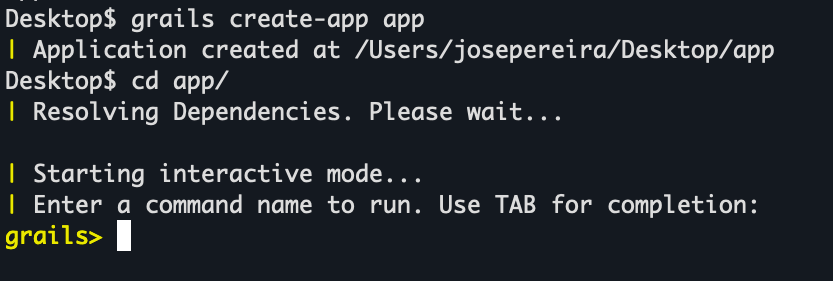
\includegraphics[scale=0.45]{images/grails-1.png}
    \caption{Criação da aplicação, e inicialização do interpretador da framework \textbf{Grails}.}
    \label{fig:grails-1}
\end{figure}

\begin{figure}[H]
    \centering
    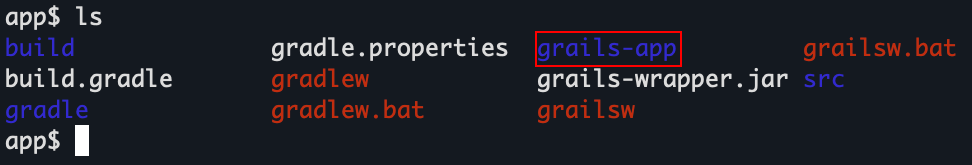
\includegraphics[scale=0.50]{images/grails-2.png}
    \caption{Estrutura do projeto criada após execução do comando \textit{grails create-app nome-app}.}
    \label{fig:grails-2}
\end{figure}

\hspace{5mm} Após a criação da aplicação, executa-se o comando \textit{grails}, para aceder ao interpretador. A execução da aplicação, faz-se através do interpretador, com o comando \textit{run-app}, tal como se pode observar na figura \ref{fig:grails-6}. A aplicação acede-se via browser no \textit{localhost}, porta 8080, onde aparecerá, uma página da \textit{Grails}, sendo possível ver os controllers existentes, tal como se pode observar na figura \ref{fig:grails-7}. 


\begin{figure}[H]
    \centering
    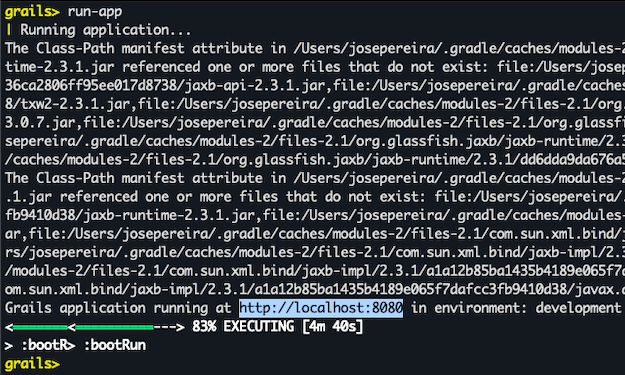
\includegraphics[scale=0.50]{images/grails-6.png}
    \caption{Execução da aplicação web, através do interpretador.}
    \label{fig:grails-6}
\end{figure}

\hspace{5mm} A diretoria mais importante é a \textit{graisl-app}, onde se encontram todos os sources files \textbf{Grovvy}. Nesta diretoria, os ficheiros são divididos em diferentes sub-diretorias (camadas), de forma automática pela framework. Na figura \ref{fig:grails-3}, pode-se verificar com mais detalhe a composição desta diretoria, onde se assinala a quadrados vermelhos as camadas \textbf{MVC}.

\begin{figure}[H]
    \centering
    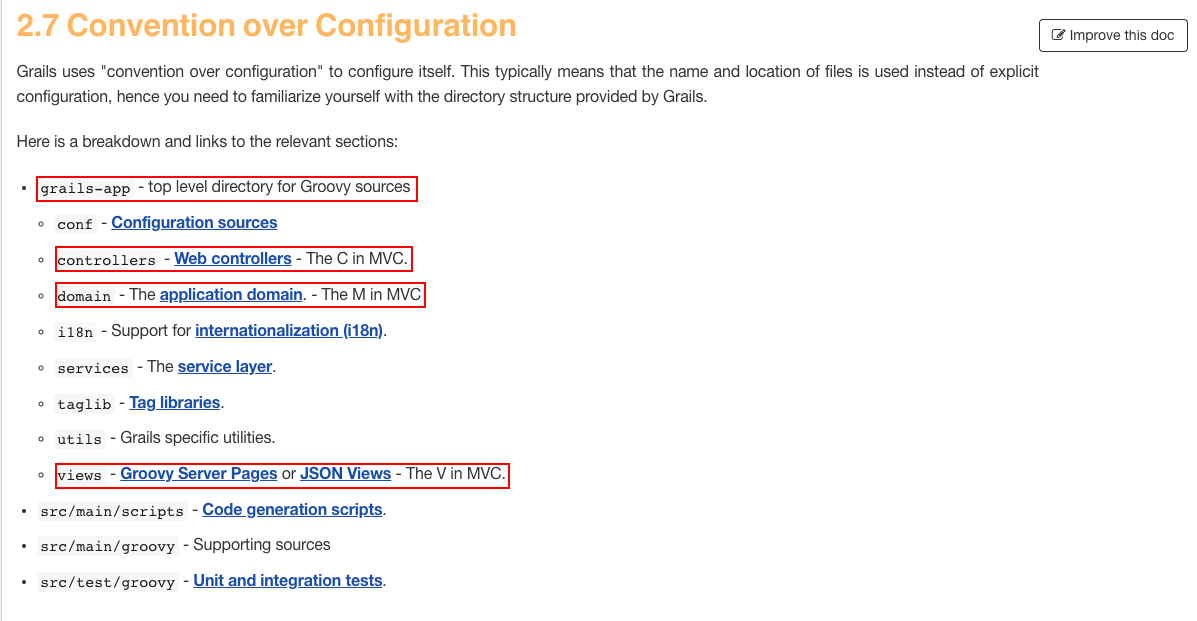
\includegraphics[scale=0.50]{images/grails-3.png}
    \caption{Composição da diretoria \textit{grails-app}, distribuindo as várias camadas, por diferentes diretorias.}
    \label{fig:grails-3}
\end{figure}

\hspace{5mm} No entanto, poderá-se pensar que o programador terá o trabalho de colocar os diferentes ficheiros, nas diferentes pastas. A resposta é "não", a própria framework tal como já foi dito, faz isso. Na verdade, para se criar um \textit{Controller}, faz-se através do interpretador (figura \ref{fig:grails-4}), e desta forma, a framework consegue controlar e organizar as diferentes camadas. 

\hspace{5mm} Após a criação do controlador, é criada a classe do mesmo, na diretoria \textit{controllers}, com o sufixo \textit{Controller} ao nome dado na criação. A classe gerada, contém um método padrão, denominado \textit{index}, que corresponde a uma ação (figura \ref{fig:grails-5}), sendo que um controlador pode ter várias ações, ou seja, vários métodos.  

\begin{figure}[H]
    \centering
    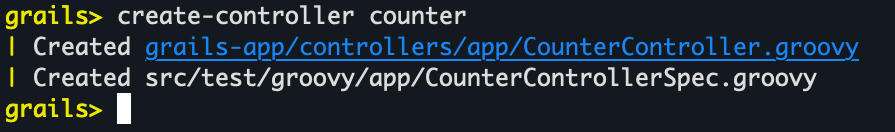
\includegraphics[scale=0.50]{images/grails-4.png}
    \caption{Criação do controller denominado \textit{Counter}.}
    \label{fig:grails-4}
\end{figure}

\begin{figure}[H]
    \centering
    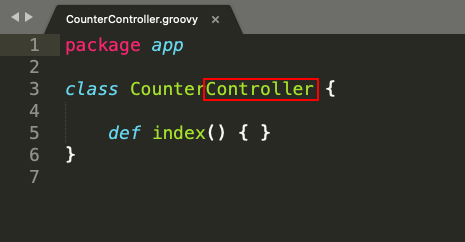
\includegraphics[scale=0.50]{images/grails-5.png}
    \caption{Classe criada automaticamente pela framework, onde é adicionado um sufixo de \textit{Controller} e um método padrão, denominado index.}
    \label{fig:grails-5}
\end{figure}

\hspace{5mm} A seguir, à criação do controlador, o mesmo já fica visível na homepage da aplicação web (figura \ref{fig:grails-7}). A forma de aceder ao controlador e às respetivas ações, segue o seguinte padrão http://localhost:8080/\textcolor{red}{controller-name}/\textcolor{blue}{action} (no caso de argumentos http://localhost:8080/\textcolor{red}{controller-name}/\textcolor{blue}{action}?agr1=value1).

\hspace{5mm} Daqui advém, os pontos fortes desta framework, para além da separação das camadas MVC, vistas anteriormente, a redução da complexidade, pois compara-se o nome do URL, com o nome do método, sabendo o método a executar, não sendo necessárias anotações ou outras alternativas, presentes em outras frameworks. Do mesmo modo, pedidos do tipo \textbf{GET} com argumentos, também se tornam simples, pois basta o método receber os argumentos com o mesmo nome dado no URL, tal como se pode observar na figura \ref{fig:grails-8} e \ref{fig:g-4} da ação \textit{set}.

\begin{figure}[H]
    \centering
    
\includegraphics[scale=0.30]{images/grails-7.png}
    \caption{Aplicação web, página inicial, com lista de controllers disponíveis.}
    \label{fig:grails-7}
\end{figure}

\hspace{5mm} Assim, após a perceção do funcionamento dos controllers, desenvolvemos várias ações para o mesmo controller, tal como se pode verificar, na figura \ref{fig:grails-8}.

\hspace{5mm} Importante realçar que o método \textit{render}, envia as strings ou valores para uma view criada automaticamente, caso esta ainda não exista, ou seja, a framework abstrai o desenvolvedor desse processo, tornando-o simples. De seguida, apresentamos os vários outputs para as diversas ações definidas, nas figuras, \ref{fig:g-1}, \ref{fig:g-2}, \ref{fig:g-3} e \ref{fig:g-4}.

\begin{figure}[H]
    \centering
    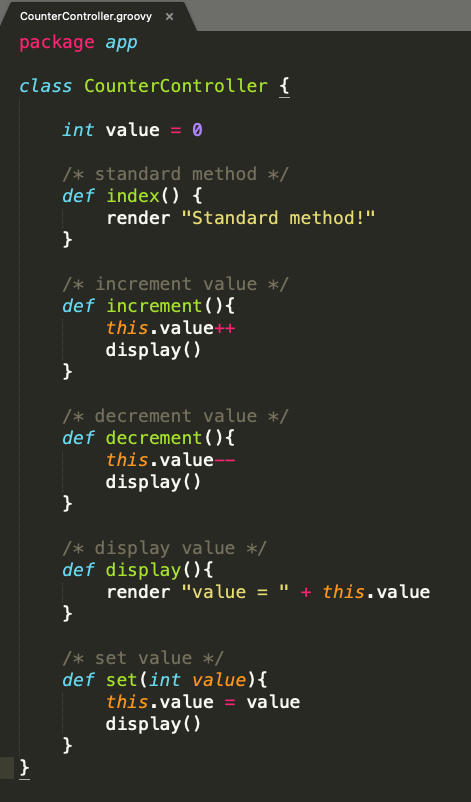
\includegraphics[scale=0.50]{images/grails-8.png}
    \caption{Controller com mais ações definidas.}
    \label{fig:grails-8}
\end{figure}

\begin{figure}[H]
    \centering
    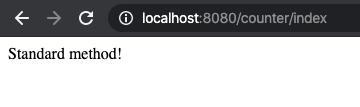
\includegraphics[scale=0.50]{images/g-1.png}
    \caption{Execução da ação index.}
    \label{fig:g-1}
\end{figure}

\begin{figure}[H]
    \centering
    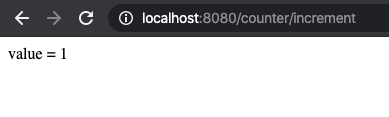
\includegraphics[scale=0.50]{images/g-2.png}
    \caption{Execução da ação increment.}
    \label{fig:g-2}
\end{figure}

\begin{figure}[H]
    \centering
    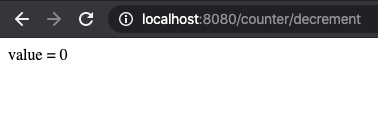
\includegraphics[scale=0.50]{images/g-3.png}
    \caption{Execução da ação decrement.}
    \label{fig:g-3}
\end{figure}

\begin{figure}[H]
    \centering
    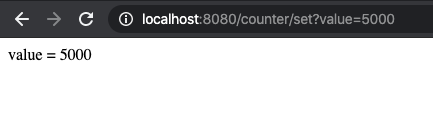
\includegraphics[scale=0.50]{images/g-4.png}
    \caption{Execução da ação set.}
    \label{fig:g-4}
\end{figure}

\hspace{5mm} Assim, conclui-se em relação à framework \textbf{Grails}, que faz uma boa divião das camadas MVC, bem como de outros níveis da aplicação, tornando-as independentes. Também importante realçar a característica de redução de complexidade e simplicidade desta framework.





